\documentclass[xcolor=pdftex,x11names,table,hyperref]{beamer}

\usepackage{verbatim}
\usepackage{setspace}
\usepackage{url}
\usepackage{xcolor} % See documentation PDF at http://www.ctan.org/pkg/xcolor
\definecolor{darkgreen}{rgb}{0,0.3,0}
\definecolor{darkblue}{rgb}{.05,.05,.30}
\definecolor{lightgrey}{rgb}{0.65,0.65,0.65}
\usepackage{tikzsymbols}


\setbeamertemplate{section in toc}[sections numbered]
\setbeamertemplate{subsection in toc}[subsections numbered]
\setbeamertemplate{subsubsection in toc}[subsubsections numbered]
\usetheme{Singapore}
\setbeamertemplate{navigation symbols}{}
\setbeamertemplate{footline}{%
\vspace{0.0em}%
\hspace{0.5em}%
{\color[rgb]{.1,.1,.1} \insertframenumber{}~/~\inserttotalframenumber}
}

\newcommand{\code}[1]{{\color{darkgreen}\texttt{#1}}}
\newcommand{\detail}[1]{{\color{lightgrey}\small{}#1}}
\newcommand{\teeny}[1]{\scalebox{0.09}{#1}}
\newcommand{\tablecolors}{\rowcolors{2}{blue!12}{white}} % Cool table colors


\begin{document}

\title{Sequence to Sequence Models \\[1.5em]
 %
\includegraphics[width=0.5\textwidth]{images/kitten_string_flickr_albaraa.jpg} \\[-1.0em]
 %\small{Possibilities} \\[1.0em]
 %LT1 \\[1.0em]
 }
\author{\href{http://jon.dehdari.org}{Jon Dehdari}}
\frame{\titlepage}

\begin{frame}{Good Morning!}
	\begin{center}
	%\includegraphics[width=0.8\textwidth]{images/.jpg}
	\end{center}
\end{frame}


% Cho: It's all LMs! (ala doc brown)
% ?Joint model?

% Start with basic seq2seq model
% http://arxiv.org/abs/1409.3215 (Sutskever et al, 2014)
% can use final hidden layer to kinda represent entire sentence.  Shortcomings?
\begin{frame}{Sentence Vectors}
\begin{itemize}
	\item We've seen that words can be represented as vectors. Can sentences be represented as vectors? \pause
	\item Sure, why not? \pause How?  From the hidden state at the end of a sentence: \hspace{1.0em}
	$ \mathbf{h}_i = \phi_{\text{enc}} ( \mathbf{h}_{i-1}, \mathbf{s}_i ) $
		\small{ \detail{($\phi_{\text{enc}}$ = LSTM or GRU)} }
	\pause
	\begin{center} 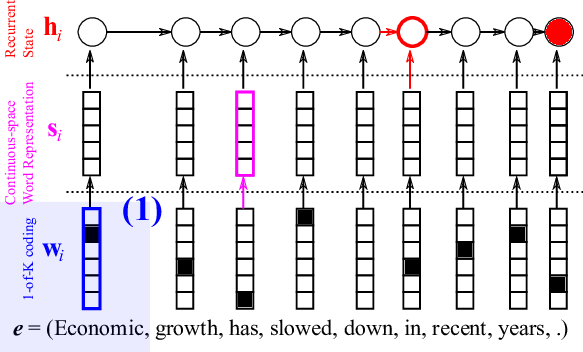
\includegraphics[width=0.63\textwidth]{images/cho_nvidia_fig-3_one-hot.png} \end{center}
	\pause
	\item Are they any good?  For Elman networks (SRNs), not so much.  For LSTMs or GRUs, yes, they're pretty good
\end{itemize}
\teeny{Images courtesy of \url{http://devblogs.nvidia.com/parallelforall/introduction-neural-machine-translation-gpus-part-2}}
\end{frame}

\begin{frame}{Sentence Vector Examples}
\hspace*{-3.0em}%
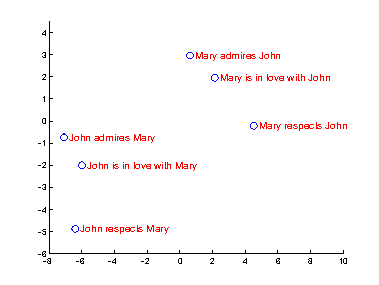
\includegraphics[width=0.60\textwidth]{images/sutskever-etal2014_fig2a.pdf}\hspace*{-1.0em}%
	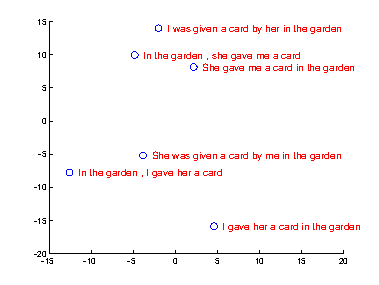
\includegraphics[width=0.60\textwidth]{images/sutskever-etal2014_fig2b.pdf}
\teeny{Images courtesy of \href{http://arxiv.org/abs/1409.3215}{Sutskever, et al (2014)}}
\end{frame}

% generate text from a vector (decoding)
\begin{frame}{Generating Sentences from Vectors}
\begin{itemize}
	\item We can also try to go the other direction, generating sentences from vectors
	\item How?  Use an RNN to \textbf{decode}, rather than \textbf{encode} a sentence: \hspace{1.0em}
		$ \mathbf{z}_i = \phi_{\text{dec}} ( \mathbf{z}_{i-1}, \mathbf{u}_{i-1}, \mathbf{h}_T ) $
\begin{center}
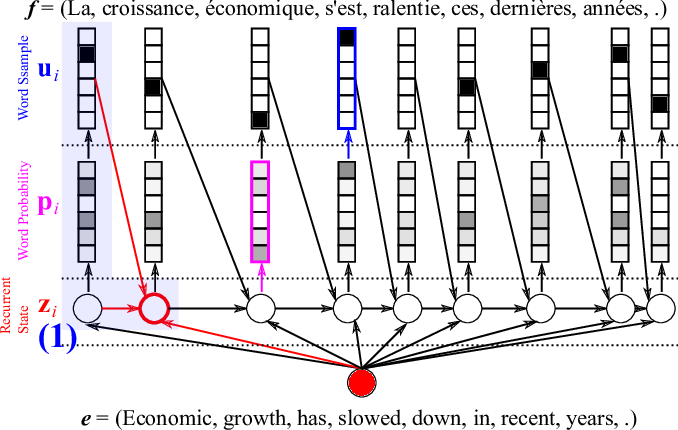
\includegraphics[width=0.60\textwidth]{images/cho_nvidia_figure7_internal-hidden-state.png}\hspace*{-1.0em}%
\end{center}
	\item $\mathbf{h}_T$ ensures global sentence coherency (\& adequacy in MT); $\mathbf{u}_{i-1}$ ensures local fluency
\end{itemize}
\teeny{Images courtesy of \url{http://devblogs.nvidia.com/parallelforall/introduction-neural-machine-translation-gpus-part-2}}
\end{frame}



% http://devblogs.nvidia.com/parallelforall/introduction-neural-machine-translation-gpus-part-2/
% https://www.tensorflow.org/versions/master/tutorials/seq2seq/index.html
\begin{frame}{Using Neural Encoders \& Decoders to Translate}
\begin{itemize}
	\item We can combine the neural encoder and decoder of previous slides to form an \textbf{encoder-decoder model}
	\item This can be used for machine translation, and other tasks that map sequences to sequences
\begin{center}
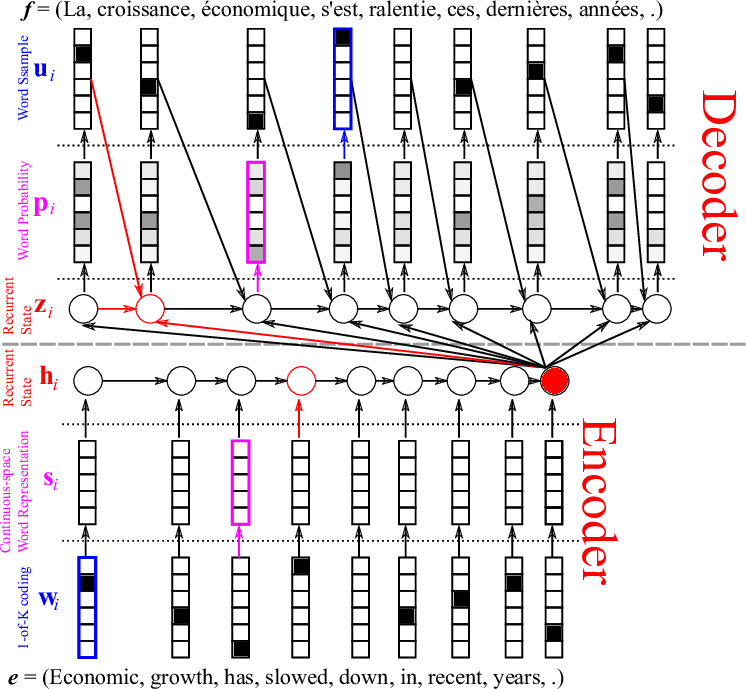
\includegraphics[width=0.60\textwidth]{images/cho_nvidia_fig-2_enc-dec.png}\hspace*{-1.0em}%
\end{center}
\end{itemize}
\end{frame}



% bidirectional RNNs
\begin{frame}{Bidirectional RNNs}
\begin{itemize}
	\item 
	\item 
\end{itemize}
\end{frame}


% attention
\begin{frame}{Pay Attention!}
\begin{itemize}
	\item 
	\item 
\end{itemize}
\end{frame}



% image caption generation
% http://www.wildml.com/2015/09/recurrent-neural-networks-tutorial-part-1-introduction-to-rnns/
\begin{frame}{Image Caption Generation}
\begin{itemize}
	\item 
	\item 
\end{itemize}
\end{frame}




\begin{frame}{}
\begin{itemize}
	\item 
	\item 
\end{itemize}
\end{frame}





% \begin{frame}{}
% \begin{itemize}
% 	\item 
% 	\item 
% 	\item 
% \end{itemize}
% \end{frame}


\end{document}
